%%%%%%%%%%%%%%%%%%%%%%%%%%%%%%%%%%%%%%%%%%%%%%%%%%%%%%%%%%%%%%%%%%%%%%%%%%%%
%% Trim Size: 9.75in x 6.5in
%% Text Area: 8in (include Runningheads) x 5in
%% ws-ijfcs.tex: 05-05-2015
%% Tex file to use with ws-ijfcs.cls written in Latex2E.
%% The content, structure, format and layout of this style file is the
%% property of World Scientific Publishing Co. Pte. Ltd.
%% Copyright 2015 by World Scientific Publishing Co.
%% All rights are reserved.
%%%%%%%%%%%%%%%%%%%%%%%%%%%%%%%%%%%%%%%%%%%%%%%%%%%%%%%%%%%%%%%%%%%%%%%%%%%%
%

\documentclass{ws-ijfcs}
\usepackage{enumerate}
\usepackage{textcomp}
\usepackage{url}
\usepackage{graphicx}
\usepackage[numbers]{natbib}
\usepackage{bussproofs}
\usepackage{tikz}
\usepackage{amssymb}
\usepackage{amsmath}
\usepackage[all,cmtip]{xy}
\usetikzlibrary{positioning, automata}
\usetikzlibrary{decorations.pathmorphing}
 \usetikzlibrary{snakes}


\tikzset{snake it/.style={decorate, decoration=snake}}
\urlstyle{same}
\begin{document}

\markboth{E. Shemetova, A. Okhotin, S. Grigorev}
{Rational index of bounded-oscillation languages}

%%%%%%%%%%%%%%%%%%%%% Publisher's Area please ignore %%%%%%%%%%%%%%%
%
\catchline{}{}{}{}{}
%
%%%%%%%%%%%%%%%%%%%%%%%%%%%%%%%%%%%%%%%%%%%%%%%%%%%%%%%%%%%%%%%%%%%%

\title{Rational index of bounded-oscillation languages\footnote{
This research was supported by the Russian Science Foundation, grant \textnumero 18-11-00100.}}
%using \LaTeX\footnote{For the title, try not to use more than 3
%lines. Typeset the title in 10 pt Roman, boldface with the first letter of
%important words capitalized.}}%

\author{Ekaterina Shemetova\footnote{
St. Petersburg State University, 
7/9 Universitetskaya nab., Saint Petersburg 199034, Russia.}
\footnote{
St. Petersburg Academic University, 
ul. Khlopina, 8, Saint Petersburg 194021, Russia.}
\footnote{
JetBrains Research,
Primorskiy prospekt 68-70, Building 1, St. Petersburg, 197374, Russia.}
}

\address{
\email{katyacyfra@gmail.com}}

\author{Alexander Okhotin\footnotemark[2] }

\address{
\email{alexander.okhotin@spbu.ru}
}

\author{Semyon Grigorev\footnotemark[2] \footnotemark[4] }

\address{
\email{s.v.grigoriev@spbu.ru}
}


\maketitle

\begin{history}
\received{(Day Month Year)}
%\revised{(Day Month Year)}
\accepted{(Day Month Year)}
%\comby{(xxxxxxxxxx)}
\end{history}

\begin{abstract}
The rational index of a context-free language  $L$ is a function $f(n)$, such that for each regular language $R$ recognized by an automaton with $n$ states, the intersection of $L$ and $R$ is either empty or contains a word shorter than $f(n)$. It is known that the context-free language (CFL-)reachability problem and Datalog query evaluation for context-free languages (queries) with the polynomial rational index is in NC, while these problems is P-complete in the general case. We investigate the rational index of bounded-oscillation languages and show that it is of polynomial order. We obtain upper bounds on the values of the rational index for general bounded-oscillation languages and for some of its previously studied subclasses.
\end{abstract}

\keywords{bounded-oscillation languages; rational index; CFL-reachability; parallel complexity; context-free languages; Datalog programs; context-free path queries.}

\section{Introduction}
\label{intro}
The notion of a rational index was introduced by Boasson et al. \cite{RatBasic} as a complexity measure for context-free languages.  The rational index $\rho_L(n)$ is a function, which denotes the maximum length of the shortest word in $L \cap R$, for arbitrary $R$ recognized by an $n$-state automaton. The rational index plays an important role in determining the parallel complexity of such practical problems as the context-free language (CFL-)reachability problem and Datalog chain query evaluation.

The CFL-reachability problem for a fixed context-free grammar $G$ is stated as follows: given a directed edge-labeled graph $D$ and a pair of nodes  $u$ and $v$, determine whether there is a path from $u$ to $v$ labeled with a string in $L(G)$.  That is, CFL-reachability is a kind of graph reachability problem with path constraints given by context-free languages. It is an important problem underlying some fundamental static code analysis like data flow analysis and program slicing \cite{RepsBasic}, alias analysis \cite*{Chatterjee, alias}, points-to analysis \cite{Incremental} and other \cite{Cai, android, typeflow}, and graph database query evaluation \cite{Azimov, GrigorevRagozina, HellingsCFPQ, RDF}.  


The Datalog chain query evaluation on a database graph is equivalent to the CFL-reachability problem. 
\begin{example}[Datalog query as a context-free grammar]
\label{DatalogExample}
Consider a database  $D$ with relation ``$child$''. It also can be represented as a digraph $G$, where each node of the graph corresponds to a person, and edges are labeled with a word ``$child$''.


The following Datalog query determines all pairs of people $x$ and $y$ such that $x$ is a descendant of $y$: 


$Desc(x, y)$ :- $Child(x, y)$

$Desc(x, y)$ :- $Child(x, z), Desc(z, y)$


This query can be represented as a context-free grammar with the following rules: 


$Desc \rightarrow Child$ $\vert$ $Child$ $Desc$


$Child  \rightarrow child$


Thus, evaluating the above mentioned Datalog query over database $D$ is equivalent to solving the CFL-reachability problem for a context-free grammar representation of this query and the edge-labeled graph $G$.
\end{example}



Unlike context-free language recognition, which is in NC (when context-free grammar is fixed), the CFL-reachability problem is P-complete \cite{ PCompl, RepSeq,  Yannakakis}. Practically, it means that there is no efficient parallel algorithm for solving this problem (unless P $\neq$ NC). 


The question on the parallel complexity of Datalog chain queries was investigated independently \cite{ChainQ, Vardi, Ullman}. Ullman and Van Gelder \cite{Ullman} introduce the notion of a \textit{polynomial fringe property} and show that chain queries having this property is in NC. The polynomial fringe property is equivalent to having the polynomial rational index: for a context-free language $L(G)$ having the polynomial rational index $\rho_L(n) = poly(n)$, where $poly(n)$ is some polynomial, is the same as for corresponding query to have the polynomial fringe property. It has been shown that for every algebraic number $\gamma$, a language with the rational index in $\Theta (n^\gamma )$ exists \cite{GreibRat}.  In contrast, the rational index of languages, which generate all context-free languages (an example of such language is the Dyck language on two pairs of parentheses $D_2$) is in order $exp(\Theta(n^2/\ln n))$ \cite{CFRat}, and, hence, this is the upper bound on the value of the rational index for every context-free language.


While both problems is not parallelizable in general, it is useful to develop more efficient parallel solutions for specific subclasses of the context-free languages. For example, there are context-free languages which admit more efficient parallel algorithms in comparison with the general case of context-free recognition \cite{IBARRA2, IBARRA, Okhotin2014ComplexityOI}.  The same holds for the CFL-reachability problem: there are some examples of context-free languages, for which the CFL-reachability problem lies in NL complexity class (for example, linear and one-counter languages) \cite{labelledGraphs, LReach, Regularrealizability, VyalyiRR}. These languages have the polynomial rational index.


The family of linear languages (linear Datalog programs, respectively) is the well-known subclass of context-free languages having the polynomial rational index \cite{RatBasic, Ullman}. The value of its rational index is in $O(n^2)$ \cite{RatBasic}. Linear Datalog programs have been widely studied by deductive database community, because efficient evaluation methods and optimisation techniques exist for such programs \cite{linearisability, linopt, Ullman}. For instance, the Datalog program in Example~\ref{DatalogExample} is linear. Many efforts have been devoted to find larger subclasses of context-free languages (Datalog programs) having the polynomial rational indices \cite{ChainQ, linearisability, RatBasic, KanellakisParallel, Regularrealizability, Ullman, VyalyiRR}.  Two equivalent classes generalizing linear languages were proposed: piecewise linear programs \cite{KanellakisParallel, Ullman} and the family of quasi-rational languages (the substitution closure of the family of linear languages) \cite{RatBasic}; both were independently shown to have the polynomial rational index. Quasi-rational languages are generated by \textit{nonexpansive} grammars. A variable $S$ in a context-free grammar $G$ is expansive if there exists a derivation $S  \stackrel {*}{\Rightarrow } uSvSw$ for some words $u, v, w$. A grammar which contains no expansive variable is said to be nonexpansive. However, it was shown by Afrati et al. that piecewise linear programs is equivalent to linear programs \cite{linearisability}. Therefore, the generalization of linear languages preserving polynomiality of the rational index is remain to be found.


In this work we investigate the rational index of  bounded-oscilation languages. Bounded-oscillation languages were introduced by Ganty and Valput \cite{BoundOsc}. Just like linear languages, it is defined by restriction on the pushdown automata. This restriction is based on the notion of \textit{oscillation}, a special measure of how the stack height varies over time. This class generalizes a fimily of linear languages.


\textbf{Our contributions.} Our results can be summarized as follows:
\begin{itemize}
\item We show that the rational index of bounded-oscillation languages of Ganty and Valput \cite{BoundOsc} is polynomial and give an upper bound on its value in dependence of the value of oscillation.
\item We give upper bounds on the value of rational indices of previously studied subclasses of bounded-oscillation languages: superlinear and ultralinear languages.
\end{itemize}
\section{Preliminaries}

In this section we introduce common definitions in graph theory and formal language theory which will be used in this paper. 
Also, we provide brief description of Azimov's algorithm which is used as a base of our solution.

\subsection{Graphs}

In this work we use edge-labelled digraph as a data model and define it as follows.
\begin{definition} \emph{Labeled directed graph} is a triple $D = (V,E,\sigma)$, where
\begin{itemize}
    \item $V$ is a set of vertices
    \item $E$ is a set of edges
    \item $\sigma \subseteq \Sigma$ is a set of labels, and a set of edges $E\subseteq V\times \sigma \times V$
\end{itemize}
\end{definition}

An example of the graph is presented in figure~\ref{fig:example_input_graph}.

\begin{figure}[h]
    \centering        
    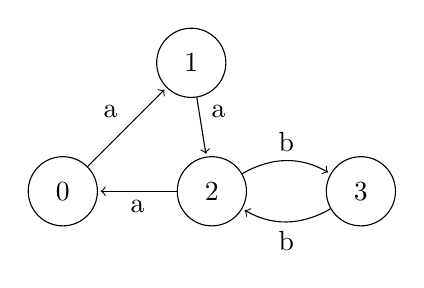
\begin{tikzpicture}[shorten >=1pt,auto]
       \node[state] (q_0)                      {$0$};
       \node[state] (q_1) [above right=of q_0] {$1$};
       \node[state] (q_2) [right=of q_0]       {$2$};
       \node[state] (q_3) [right=of q_2]       {$3$};
        \path[->]
        (q_0) edge  node {a} (q_1)
        (q_1) edge  node {a} (q_2)
        (q_2) edge  node {a} (q_0)
        (q_2) edge[bend left, above]  node {b} (q_3)
        (q_3) edge[bend left, below]  node {b} (q_2);
    \end{tikzpicture}
    \caption{The example of input graph $\mathcal{G}$}
    \label{fig:example_input_graph}
\end{figure}

We use adjacency matrix decomposed to a set of a boolean matrix as a representation of the graph.
\begin{definition}
An adjacency matrix $M$ of the graph $\mathcal{G}=$ is a square $|V|\times|V|$ matrix, such that $M[i,j] = \{l \mid e = (i,l,j) \in E\}$.
\end{definition}

Adjacency matrix $M$ of the graph $\mathcal{G}$ is

$$
    M =
    \begin{pmatrix}
    . & \{a\} & . & .     \\
    . & . & \{a\} & .     \\
    \{a\} & . & . & \{b\} \\
    . & . & \{b\} & .
    \end{pmatrix}.
$$

\begin{definition}

Boolean decomposition of adjacency matrix $M$ of graph $\mathcal{G}=$ is set of Boolean matrix $$\mathcal{M} = \{M^l \mid l \in L, M^l[i,j]=1 \iff l \in M[i,j]\}.$$

\end{definition}

Matrix $M$ can be represented as a set of two Boolean matrices $M^a$ and $M^b$ where
\begin{align}
M^{a} =
\begin{pmatrix}
    . & 1 & . & .   \\
    . & . & 1 & .   \\
    1 & . & . & .   \\
    . & . & . & .  
\end{pmatrix}, 
M^{b} =
\begin{pmatrix}      
    . & . & . & .   \\
    . & . & . & .   \\
    . & . & . & 1   \\
    . & . & 1 & . 
\end{pmatrix} \label{eq:boolean_decomposition_of_graph}
\end{align}
\subsection{Languages}

\begin{definition}\emph{Context-free grammar} is a 4-tuple $G=(N, \Sigma, R, S)$, where 
\begin{itemize}
    \item $N$ is a set of nonterminals
    \item $\Sigma$ is a set of terminals
    \item $R$ is a finite set of productions of the followings form: $A \to \alpha, ~A \in N,~ \alpha \in (N \cup \Sigma)^*$
    \item $S$ - a starting nonterminal
\end{itemize}
\end{definition}

\begin{definition} \emph{Context-free language} is a language generated by a context-free grammar:
\begin{align*}
     L(G) = \{w \in \Sigma^* \mid S \Rightarrow^* w \} 
\end{align*}
Where $S \Rightarrow^* w$  denotes that a string $w$ can be generated from a starting non-terminal $S$ using some sequence of production rules from $P$.
\end{definition}

\begin{definition} Context-free grammar $G = (N, \Sigma, R, S)$ is said to be in \emph{Chomsky normal form} if all productions in $R$ are of the form:
    \begin{itemize}
        \item $A \rightarrow BC,~A,~B,~C \in N$
        \item  $A \rightarrow a,~A \in N,~a \in \Sigma$
        \item $S \rightarrow \varepsilon,~\varepsilon$ is an empty string
    \end{itemize}
\end{definition}
Note that every context-free grammar can be transformed into an equivalent one in Chomsky Normal Form. 
\begin{definition} Context-free grammar $G = (N, \Sigma, P, S)$ is said to be in \emph{Weak Chomsky normal form} if all productions in $P$ are of the form:
    \begin{itemize}
        \item $A \rightarrow BC,~A,~B,~C \in N$
        \item  $A \rightarrow a,~A \in N,~a \in \Sigma$
        \item $A \rightarrow \varepsilon,~A \in N$
    \end{itemize}
\end{definition}
In other words, weak Chomsky normal form differs from Chomsky normal Form in the followings:
\begin{itemize}
    \item $\varepsilon$ can be derived from any non-terminal
    \item $S$ can be at a right part of productions
\end{itemize}
    
    
For example, let's consider the following context-free grammar, which generates the language $L(G) = \{A^nB^n, n \in \mathbb{N}\}$:
$G=(N, \Sigma, P, S), ~N=\{S\},~\Sigma=\{A,B\}$ and productions: 
\begin{align*}
S \rightarrow AB \\
S \rightarrow ASB\\
S \rightarrow \varepsilon
\end{align*}
After transformation to Chomsky Normal Form the resulting grammar:
\begin{align*}
S \rightarrow AB \\
S \rightarrow AC \\
C \rightarrow SB \\
S \rightarrow \varepsilon
\end{align*}

This productions itself are the grammar that has the same result as original grammar.

We use a context-free grammar in the weak Chomsky Normal Form without a starting non-terminal, which will be specified in the path queries for the graph. It should be noted that we omit the rules of the form $A \rightarrow \varepsilon$ for the reason that they correspond to trivial paths, which are more convenient to consider separately.

\begin{definition}\emph{Context-free relation} is a relation $R_A \subseteq V \times V$ for graph $G = (V, E)$, context-free grammar $G = (N,~\Sigma,~P)$ and fixed non-terminal $A$:
\begin{align*}
     R_A = \{(n, m) \mid \exists n \pi m~(l(\pi) \in L(G_A))\}
\end{align*}
\end{definition}

 Now, the definition for \emph{multiple-source (single-source) context-free path querying problem} can be formulated in the introduced notation as follows. For the given graph $G = (V, E)$, context-free grammar $G=(N, \Sigma, P)$ and set of source vertices $Src$ we need to find all context-free relations $R_A$ for any $A \in Src$. 
 
\subsection{Matrix-Based Algorithm}
Let $D = (V, E)$ be the input graph and $G = (N, \Sigma, P)$ be the input grammar. For the context-free path query evaluation, we need to provide context-free relations \mbox{$R_A \subseteq V \times V$} for every \mbox{$A \in N$}.
The matrix-based algorithm for CFPQ can be expressed in terms of operations over Boolean matrices (see listing~\ref{alg:algo0}) which is an advantage for implementation.
{\footnotesize
\begin{algorithm}
\begin{algorithmic}[1]
\caption{Context-free path querying algorithm}
\label{alg:algo0}
\Function{evalCFPQ}{$D=(V,E), G=(N,\Sigma,P)$}
    \State{$n \gets$ |V|}
    \State{$T \gets \{T^{A_i} \mid A_i \in N, T^{A_i}$ is a matrix $n \times n$, $T^{A_i}_{k,l} \gets$ \texttt{false}\} }
    \ForAll{$(i,x,j) \in E$, $A_k \mid A_k \to x \in P$}
        %\Comment{Matrices initialization}
        %\For{$A_k \mid A_k \to x \in P$}
          {$T^{A_k}_{i,j} \gets \texttt{true}$}
        %\EndFor
    \EndFor
    \ForAll{$A_k \mid A_k \to \varepsilon \in P$}
        \ForAll{$i \in \{0,\ldots ,n-1\}$}
            {$T^{A_k}_{i,i} \gets \texttt{true}$}
        \EndFor
    \EndFor

    \While{any matrix in $T$ is changing}
        %\Comment{Transitive c	losure calculation}
        \For{$A_i \to A_j A_k \in P$}
          { $T^{A_i} \gets T^{A_i} + (T^{A_j} \times T^{A_k})$ } 
        \EndFor
    \EndWhile
\State \Return $T$
\EndFunction
\end{algorithmic}
\end{algorithm}
}

This CFPQ algorithm allows efficiently apply GPGPU techniques, but it solves all-pairs problem and takes unreasonable amount of memory in scenarios in which we want to find paths from a relatively small set of vertices, since it calculates a lot of redundant information.  
\section{Rational index of bounded-oscillation languages}
\label{sec:osc}
\subsection{Upper bounds on the rational index of bounded oscillation languages}
Before we consider the value of the rational index for $k$-bounded-oscillation languages, we need to prove the following.
\begin{lemma}
\label{lem:treeheight}
Let  $G = (\Sigma, N, P, S)$ be a context-free grammar in Chomsky normal form,  $D=(V, E, \Sigma)$ be a directed labeled graph with $n$ nodes. Let $w$ be the shortest string in $L(G)\cap L(D)$. Then the height of every parse tree for $w$ in $G$ does not exceed $|N|n^2$.
\end{lemma}

\begin{proof}
Consider grammar $G'$ for $L(G)\cap L(D)$. The grammar $G = (\Sigma, N', P', S')$ can be constructed from $G$ using the classical Bar-Hillel et al. \cite{BarHillel} construction: $N' \subseteq N \times V \times V $  contains all tiples $(A, i, j)$ such that $A \in N, i, j \in V$ ; $P'$ contains production rules in one of the following forms:
\begin{enumerate}
\item $(A, i, j) \rightarrow (B, i, k), (C, k, j)$ for all $(i, k, j)$ in $V$  if $A \rightarrow BC \in P$
\item $(A, i, j) \rightarrow a$ for all $(i, j)$ in $V$ if $A \rightarrow a$.
\end{enumerate}
A triple $(A, i, j)$ is \textit{realizable} iff there is a path $i\pi j$ such that $A \stackrel {*}{\Rightarrow } l(\pi)$ for some nontermimal $A \in N$. Then the parse tree $t_G$ for $w$ in $G$ can be converted into parse tree $t_{G'}$ in $G'$. Notice that every node of $t_{G'}$ is realizable triple. Also it is easy to see that the height of $t_G$ is equal to the height of $t_{G'}$. Assume that $t_{G'}$ for $w$ has a height of more than $|N|n^2$. Consider a path from the root of the parse tree to a leaf, which has length greater than $|N|n^2$. There are $|N|n^2$ unique labels $(A, i, j)$ for nodes of the parse tree, so according to the pigeonhole principle, this path has at least two nodes with the same label. This means that the parse tree for $w$ contains at least one subtree $t$ with label $(A, i, j)$ at the root, which has a subtree $t'$ with the same label. Then we can change $t$ with $t'$ and get a new string $w'$ which is shorter than $w$, because the grammar is in Chomsky normal form. But $w$ is the shortest, then we have a contradiction.

\end{proof}
From Lemma \ref{lem:treeheight} one can deduce an alternative proof of the fact that the rational index of linear languages is in $O(n^2)$ \cite{RatBasic}: the number of leaves in a parse tree in linear grammar in Chomsky normal form is proportional to its height, and thus it is in $O(n^2)$.
\begin{lemma}
\label{oscbnddim}
Let $G$ be a grammar $G = (\Sigma, N, P, S)$ in Chomsky normal form, such that every parse tree $t$ has $dim(t) \le d$, where $d$ is some constant. Let $D=(V, E, \Sigma)$ be a directed labeled graph with $n$ nodes. Then $\rho_{L(G)}$ is in $O(h^d)$ in the worst case.
\end{lemma}
\begin{proof}
Proof by induction on dimension $dim(t)$.
\\
\textbf{Basis.} $dim(t) = 1$.
\\
Consider a tree $t$ with the dimension $dim(t) = 1$. The root of the tree has the same dimension and has two children (because the grammar is in Chomsky normal form). There are two cases:  first, when both of child nodes have dimension equal to 0, then the tree has only two leaves, and second, when one of the children has dimension 1, and the second child has dimension 0. For the second case we can recursively construct a tree with the maximum number of leaves in the following way. Every internal node of such a tree has two children, one of which has dimension equal to 0 and therefore has only one leaf. This means that the number of leaves (and, hence, $\rho_{L(G)}$) in such a tree is bounded by its height and is in $O(h)$. 
\\
\textbf{Inductive step.} $dim(t) = d + 1$.
\\
Assume that $\rho_{L(G)}$ is at most $O(h^{d})$ for every $d$ in the worst case, where $h$ is the height of the tree. We have two cases for the root node with dimension equal to $d+1$: 1) both of children have a dimension equal to $d$, then by proposition the tree of heght $h$ has no more than $O(h^{d})$ leaves; 2) one of the children has a dimension $d + 1$, and the second child $v$ has a dimension $dim(v) \le d$. Again, a tree with the maximum number of leaves can be constructed recursively:  each node of such tree has two children $u$ and $v$ with dimensions $d+1$ and $d$ respectively (the greater the dimension of the node, the more leaves are in the corresponding tree in the worst case). By the induction assumption there are no more than $(h-1)^d + (h-2)^d + (h-3)^d + ... + 1 = O(h^{d+1})$ leaves, so the claim holds for $dim = d+1$.
\end{proof}
Combining Lemma \ref{lem:treeheight} and Lemma \ref{oscbnddim}, we can deduce the following.
\begin{corollary}
\label{finaldim}
Let $G$ be a grammar $G = (\Sigma, N, P, S)$ in Chomsky normal form, such that every parse tree $t$ has $dim(t) \le d$, where $d$ is some constant. Let $D=(V, E, \Sigma)$ be a directed labeled graph with $n$ nodes. Then $\rho_{L(G)}$ is in $O({(|N|n^2)}^d)$ in the worst case.
\end{corollary}
\begin{theorem}
\label{oscbndosc}
Let $L$ be a $k$-bounded-oscillation language with grammar $G = (\Sigma, N, P, S)$ in Chomsky normal form and $D=(V, E, \Sigma)$ be a directed labeled graph with $n$ nodes. Then $\rho_{L(G)}$ is in $O({|N|}^{2k}n^{4k})$ in the worst case.
\end{theorem}
\begin{proof}
By Lemma~\ref{boscdim}, every parse tree of bounded-oscillation language has also bounded dimension. Then the maximum value of the dimension of every parse tree of $k$-bounded-oscillation language is $2k$. By Corrolary~\ref{finaldim}, $\rho_{L(G)}$ is in $O({(|N|n^2)}^d)$ and, thus, $\rho_{L(G)}$ does not exceed $O({(|N|n^2)}^{2k}) = O({|N|}^{2k}n^{4k})$.
\end{proof}

As we can see from the proof of Lemma~\ref{oscbnddim}, the family of linear languages is included in the family of bounded-oscillation languages. The reason is that the family of bounded-oscillation languages generalizes the family of languages accepted by finite-turn pushdown automata \cite{BoundOsc}. It is interesting that for general PDA, particularly for $D_2$, the value of osciillation is not constant-bounded: it depends on the length of input and does not exeed $O(\log n)$ for the input of length $n$ \cite*{Gundermann, Wechsung}. However, for some previously studied subclasses of context-free languages,  oscillation is bounded by a constant.

\begin{subsection}{The rational indices of some subclasses of bounded-oscillation languages.} 

\paragraph{Superlinear languages.} 
A context-free grammar $G = (\Sigma, N, P, S)$ is \textit{superlinear} \cite{superlinear} if all productions of $P$ satisfy these conditions:
\begin{enumerate}
\item there is a subset $N_L \subseteq N$ such that every $A \in N_L$ has only linear productions $A\rightarrow aB$ or $A\rightarrow Ba$, where $B \in N_L$ and $a \in \Sigma$.
\item if $A \in N \setminus N_L$, then $A$ can have non-linear productions of the form $A \rightarrow BC$ where $B\in N_L$ and $C \in N$, or linear productions of the form $A\rightarrow \alpha B$ $\vert$ $B \alpha$ $\vert$ $\alpha$ for $B \in N_L$, $\alpha \in \Sigma^*$.
\end{enumerate}
A language is \textit{superlinear} if it is generated by some superlinear grammar. 
\begin{theorem} Let $G$ be a superlinear grammar. Then $\rho_{L(G)}$ is in $O(n^4)$.
\end{theorem}
\begin{proof}
From the definition of superlinear grammar $G$ it is observable that its parse trees have dimension at most 2. From 
Corrolary~\ref{finaldim}, if dimensions of all parse trees are bounded by some $k$ then the rational index $\rho_{L(G)}$ of such language is in $O(n^4)$.
\end{proof}
\end{subsection}
\paragraph{Ultralinear languages.} A context-free grammar $G = (\Sigma, N, P, S)$ is \textit{ultrealinear} if there exists a partition $\{N_0, N_1, ..., N_k\}$ of $N$ such that $S \in N_k$ and if $A \in N_i$, where $0 \le i \le k$, then $(A \rightarrow w) \in P$ implies $w \in \Sigma^*N_i\Sigma^*$ or $w \in {(\Sigma \cup N_0 \cup ... \cup N_i-1)}^*$. Such a partition is called an \textit{ultralinear decomposition}. A language is \textit{ultralinear} if it is generated by some ultralinear grammar. 


The ultralinear languages were originally defined by Ginsburg and Spanier \cite{Ginsburg1966FiniteTurnPA} as languages recognizable by finite-turn pushdown PDAs (a finite-turn PDA is a PDA with a fixed constant bound on the number of switches between push and pop operations in accepting computation paths). 

Every ultralinear language is generated by an ultralinear grammar in \textit{reduced form} \cite{WORKMAN1976188}.
\begin{definition}[The reduced form of ultralinear grammar.]
An ultralinear grammar $G = (\Sigma, N, P, S)$ is in \textit{reduced form} if its ultralinear decomposition $\{N_0, N_1, ..., N_k\}$ is in the following form:
\begin{enumerate}
\item $N_k=\{S\}$ and $S$ does not appear in the right part of any production rule
\item if $(A \rightarrow w) \in P \setminus \{S \rightarrow \varepsilon\}$ and $A \in N_i$, $0 \le i \le k$, then $w \in (\Sigma \cup N_i\Sigma \cup \Sigma N_i \cup N_jN_j')$, where $j, j' < i$.
\end{enumerate}
\end{definition}
\begin {theorem}
Let $G = (\Sigma, N, P, S)$ be an ultralinear grammar with the ultralinear decomposition $\{N_0, N_1, ..., N_k\}$. Then $\rho_{L(G)}$ is in $O(n^{2k})$.
\end{theorem}
\begin{proof}
Recall that by definition dimension of a parse tree is the height of its largest perfect subtree. Consider the maximum possible size of a perfect subtree which occurs in the parse tree in ultralinear grammar in reduced form. It is easy to see that the rules of the form $A \rightarrow BC$, where $A \in N_i, B, C \in N_{i-1}$ should be used as often as possible to construct the largest binary subtree. Therefore, if grammar has the subset of rules of the form $\{S \rightarrow AB, A \rightarrow A_1A_2, B \rightarrow B_1B_2, A_1\rightarrow A_3A_4, ..., A_i \rightarrow A_{i+2}, A_{i+3}, ...\}$, where $A, B \in N_{k-1}, A_1, A_2, B_1, B_2 \in N_{k-2}, A_3, A_4, ... \in N_{k-3}, ... , A_{i+2}, A_{i+3}, ... \in N_0$, the perfect binary subtree obtained with these rules will be of height not greater than $k$, so the maximum dimension of the parse tree in a ultralinear grammar in reduced form is $k$. By Corrolary~\ref{finaldim}  $\rho_{L(G)}$ is in $O(n^{2k})$.
\end{proof}

\section{Conclusions and open problems}
\label{sec:conc}

We have proved that the bounded-oscillation languages have the polynomial rational index. It means that the CFL-reachability problem and Datalog query evalution for these languages is in NC. This class is a natural generalization of linear languages, and possibly it comprises the largest previously known class of queries which is NC. It is interesting whether Datalog programs corresponding to these languages are linearizable (can always be transformed into linear Datalog programs).


There is a family of languages which has the polynomial rational index, but is not comparable with the linear languages: the family of one-counter languages. Moreover, it is not comparable with bounded-oscillation languages: for example, the Dyck language $D_1$ which is one-counter language, is not $k$-bounded-oscillation language for any $k$. Can this class be generalized in the same manner as linear languages with respect to the polynomiality of the rational index? One can consider the Polynomial Stack Lemma defined by Afrati et al. \cite{ChainQ}, where some restriction on the PDA stack contents are given, or investigate the properties of the family of the substitution closure of one-counter languages, which contains one-counter languages and has the polynomial rational index \cite{RatBasic}. 


%%For cite command type as \cite{1}; \cite{3,6} and \cite{2,4,6}.
%%For refcite command type as Refs.~[\refcite{1}];
%%[\refcite{1},\refcite{3}] and [\refcite{1}--\refcite{4}].


\section*{Acknowledgments}
This research was supported by the Russian Science Foundation, grant \textnumero 18-11-00100.



\bibliographystyle{ws-ijfcs}  
\bibliography{paper}
\end{document}